\chapter{Introduction}\label{ch:intro}

\section{Motivation}
\ac{GNSS} receivers should provide accurate and reliable guidance for space vehicles during launch and re-entry. Accurate guidance helps ensure safe, repeatable and cost effective access to space.

However, significant dynamics and vibrations experienced during launch and re-entry prevent \ac{GNSS} receivers from reliably tracking the signal from \ac{GNSS} satellites. This in turn prevents the receiver from providing accurate position, velocity and timing information to the spacecraft, forcing engineers to turn to inferior solution for guiding the spacecraft.

Using a modified version of the Namuru \ac{GNSS} receiver optimised for high dynamics, accurate and reliable performance can be potentially achieved during periods of significant dynamics during launch and re-entry. 

In this report, novel modifications to the receiver are analysed for their feasibility and steps for effective implementation are suggested.

\section{Problem Definition \& Project Objectives}

The University of New South Wales has been developing the Namuru family of \ac{GNSS} receivers since 2004\cite{MumfordNamuru}. The Namuru family of receivers uses a digital base-band processor implemented on a \ac{FPGA}\cite{Glennon11aquariusfirmware}. A photo of a recent incarnation of the receiver can be seen in figure \ref{fig:Namuru1}.

\begin{figure}[!htb] 
    \centering
    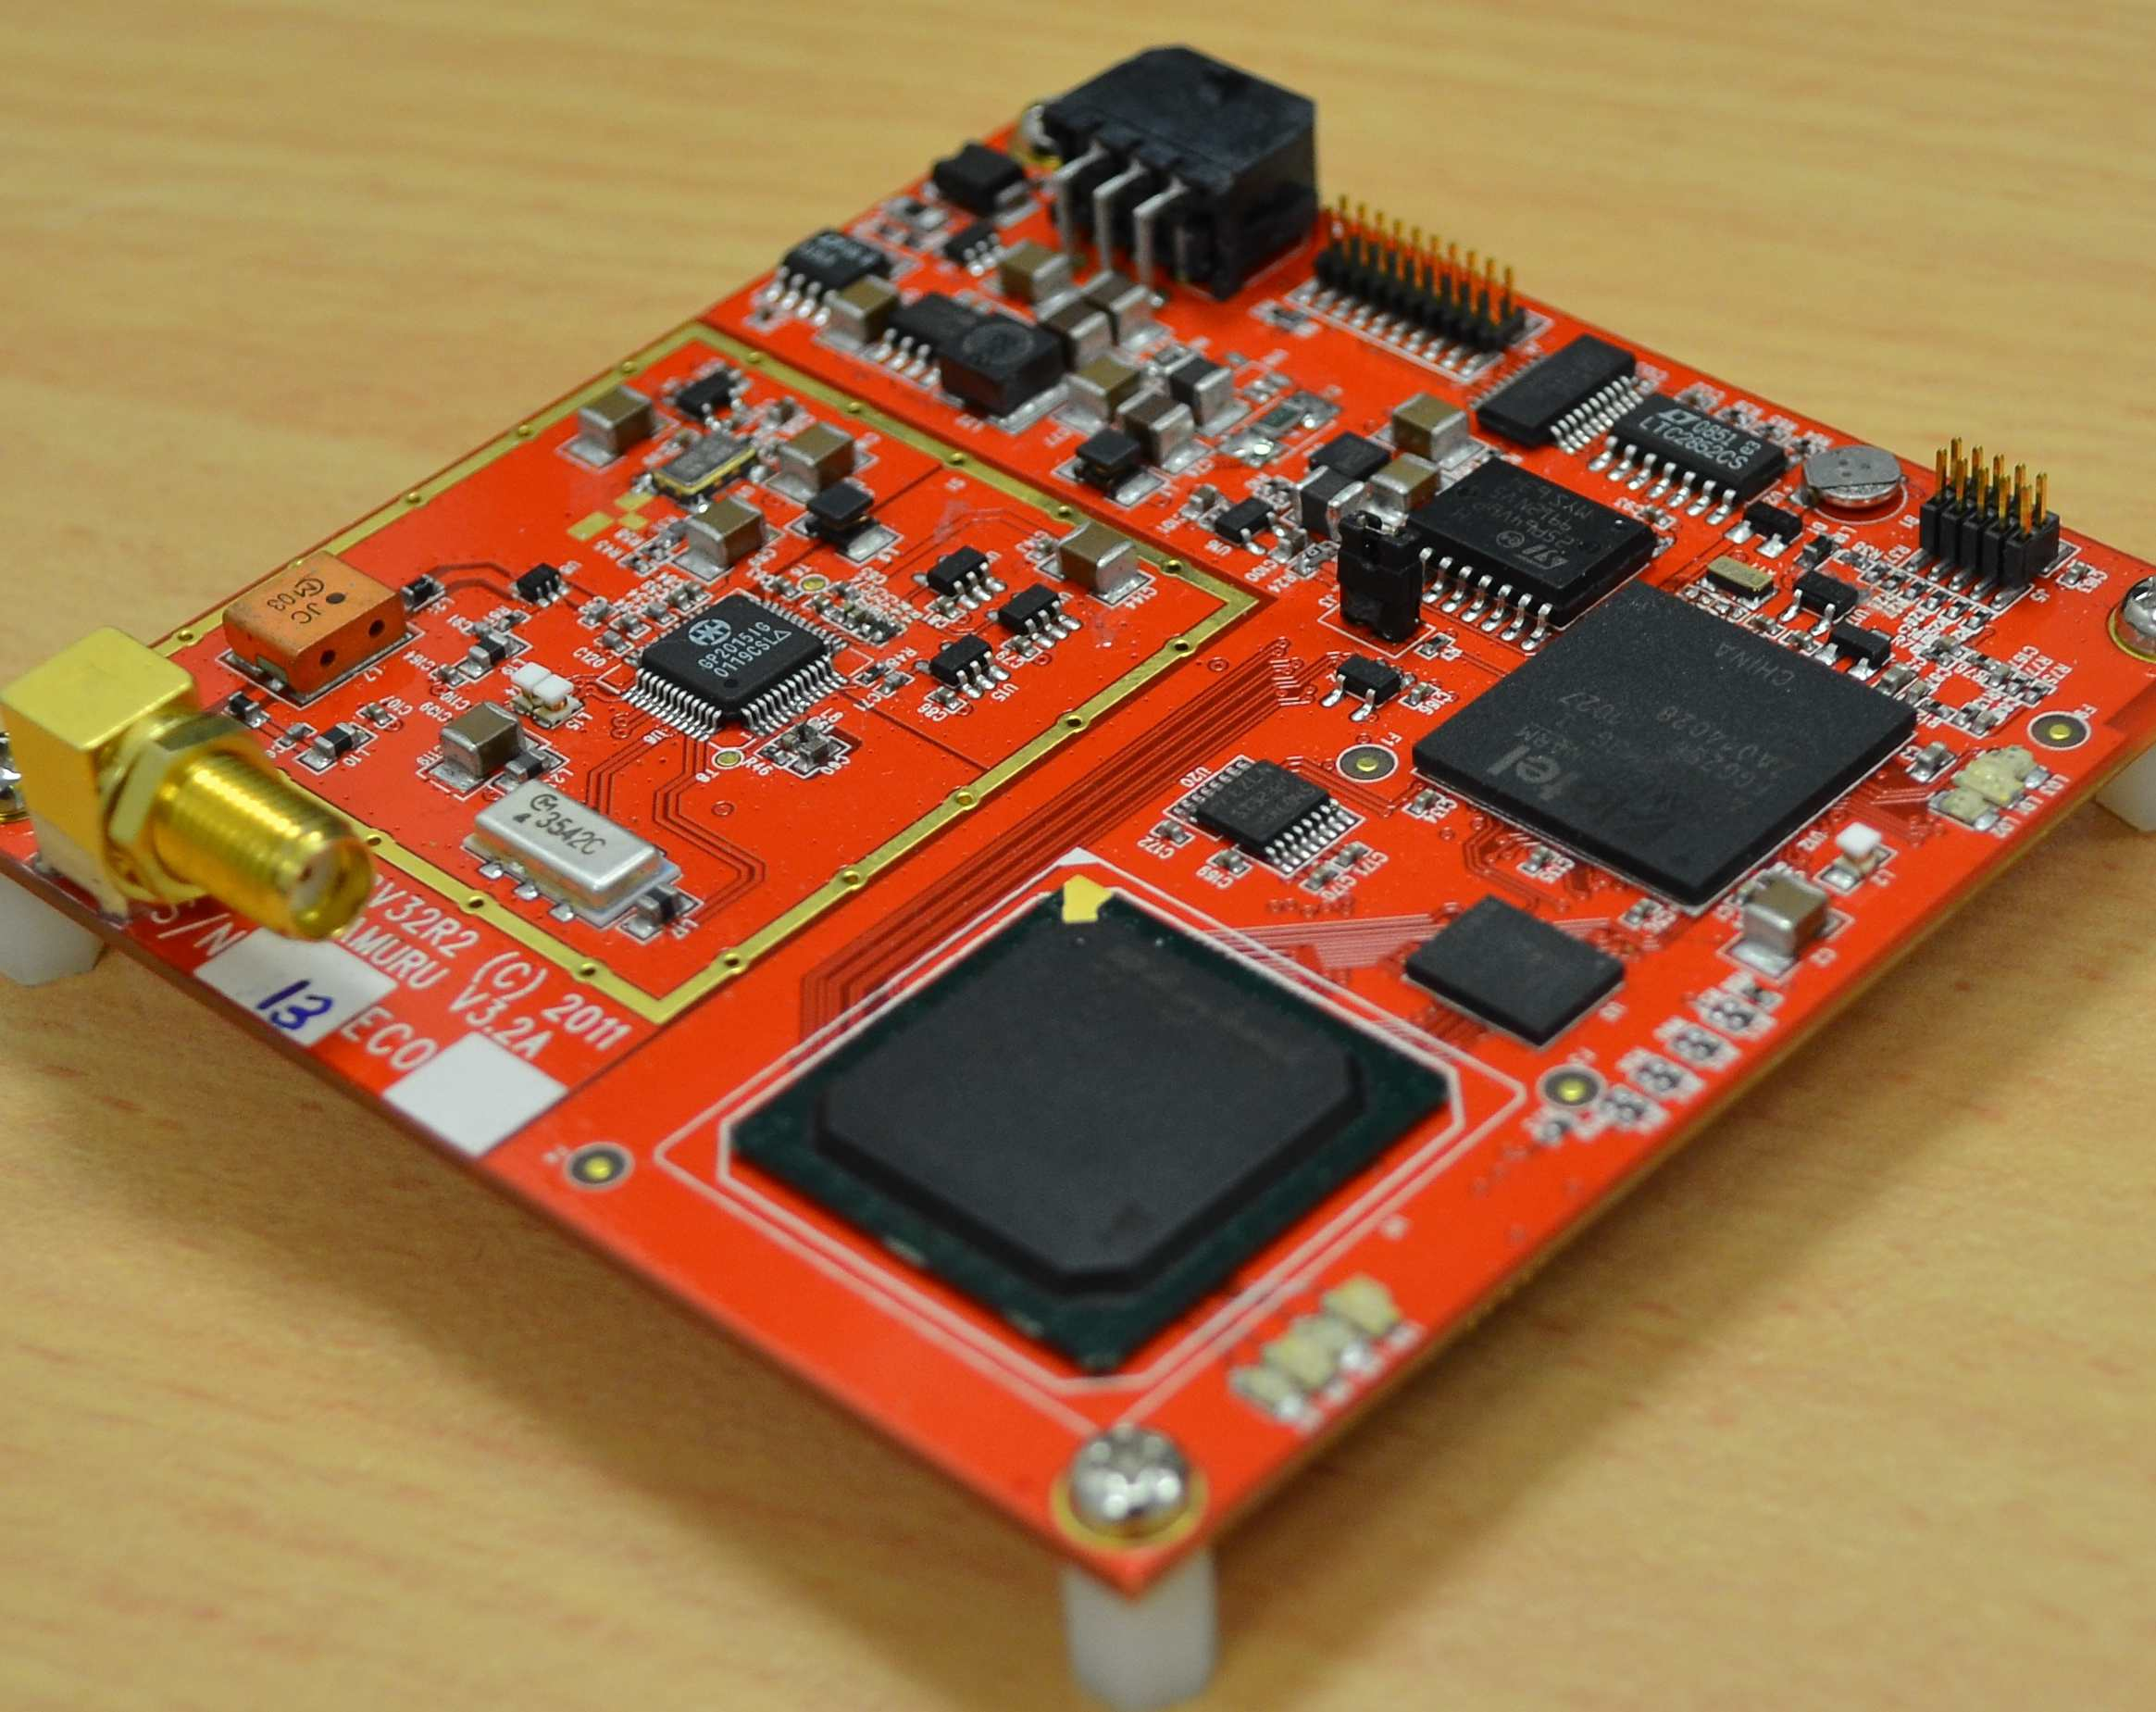
\includegraphics[width=1\textwidth]{Introduction/Namuru1.JPG} 
    \caption{The Namuru V3.2 receiver. The Zarlink GP2015 \ac{RF} front-end on the left of the board is normally covered by a \ac{RF} shield.}
    \label{fig:Namuru1}
\end{figure}

While the operation of the receiver has been validated both on land, and under simulated ballistic spaceflight conditions \cite{NamuruSpaceflight1,NamuruSpaceflight2}, the receiver is currently unable to reliably operate in high dynamics situations. 
In particular, the \ac{PLL} is unable to cope with high dynamics, and looses phase lock. This is because : 
\begin{itemize}
\item{The doppler shift due to the \ac{LOS} dynamics between the satellite and the \ac{SV}}
\item{The frequency shift in the local oscillator due to the acceleration of the quartz crystal}
\end{itemize}

The aim of this thesis is to improve the high dynamics performance of the Namuru receiver, by investigating the following issues:  

\begin{itemize}
\item{A concrete theoretical understanding of the current implementation}
\item{Validation of the existing implementation against the theory}
\item{Effect of jitter and lag on the \ac{PLL}}
\item{Alternative lock detectors and switching logic}
\item{Effects of using a direct phase controlled correlator}
\item{Implementing new techniques discussed in the literature}
\item{Effects of vibration on the \ac{PLL}}
\end{itemize}

The objectives of this thesis are as follows : 
\begin{itemize}
\item{Sustained tracking with \ac{LOS} dynamics of 15 g}
\item{Reliable operation during simulations of launch and re-entry}
\item{Reliable operation while undergoing vibration}
\end{itemize}
